\section{SVM}

\begin{frame}
	
  \centerline{\textbf{\Huge{SVM}}}
           
	\begin{figure}[ht]
	\centering
	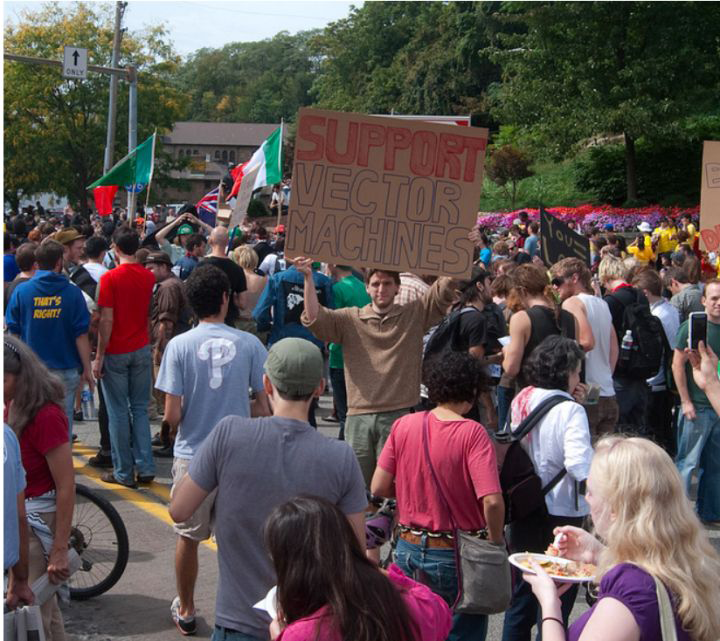
\includegraphics[width=0.5\linewidth]{partition/img/svm_0.png}  
%	\caption{this is a figure demo}
%	\label{fig:label}
	\end{figure}

\end{frame} 

\begin{frame} 
\frametitle{支持向量机}  
\begin{columns}

\column{.5\textwidth}
	\begin{itemize}
		\item SVM, 俗称支持向量机,为一种supervised learning算法,属于classification的范畴。
		\item 在数据挖掘的应用中,与unsupervised的Clustering相对应和区别。
		\item 广泛应用于机器学习(Machine Learning), 计算机视觉(Computer Vision) 和数据挖掘(Data Mining)当中。	
	\end{itemize}

\column{.5\textwidth}
	\begin{figure}[ht]
	\centering
	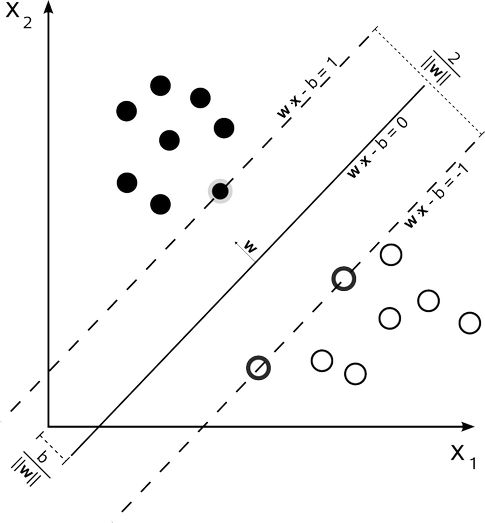
\includegraphics[width=\linewidth]{partition/img/svm_1.jpg}  
%	\caption{this is a figure demo}
%	\label{fig:label}
	\end{figure}


\end{columns}
\end{frame} 

\begin{frame}
\frametitle{一个游戏}	
现在桌子上有两种颜色的球,现在要把他们分开。
           
	\begin{figure}[ht]
	\centering
	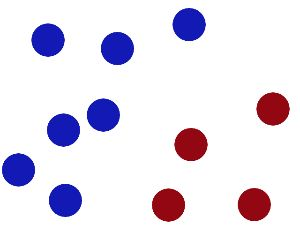
\includegraphics[width=0.5\linewidth]{partition/img/svm_2.jpg}  
%	\caption{this is a figure demo}
%	\label{fig:label}
	\end{figure}

\end{frame} 

\begin{frame}
\frametitle{一个游戏}	
我们把一根棍子放在中间,看上去干得不错。
           
	\begin{figure}[ht]
	\centering
	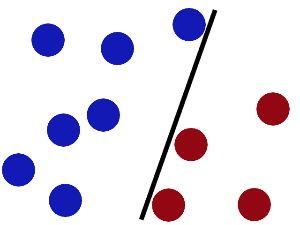
\includegraphics[width=0.5\linewidth]{partition/img/svm_3.jpg}  
%	\caption{this is a figure demo}
%	\label{fig:label}
	\end{figure}

\end{frame} 

\begin{frame}
\frametitle{一个游戏}	
有些人又往桌子上放了一些球,大部分都分对了,但是出现了一个错分的。
           
	\begin{figure}[ht]
	\centering
	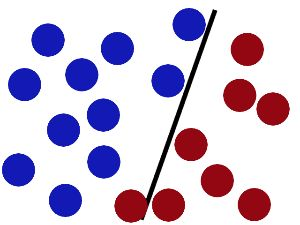
\includegraphics[width=0.5\linewidth]{partition/img/svm_4.jpg}  
%	\caption{this is a figure demo}
%	\label{fig:label}
	\end{figure}

\end{frame} 

\begin{frame}
\frametitle{一个游戏}	
SVM就是试图把棍放在最佳位置,好让在棍的两边有尽可能大的间隙。
           
	\begin{figure}[ht]
	\centering
	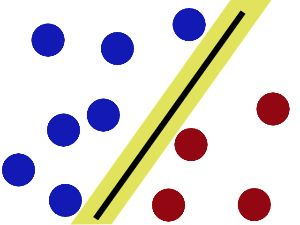
\includegraphics[width=0.5\linewidth]{partition/img/svm_5.jpg}  
%	\caption{this is a figure demo}
%	\label{fig:label}
	\end{figure}

\end{frame} 

\begin{frame}
\frametitle{一个游戏}	
现在即使放了更多的球,棍仍然是一个好的分界线
           
	\begin{figure}[ht]
	\centering
	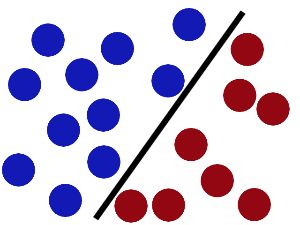
\includegraphics[width=0.5\linewidth]{partition/img/svm_6.jpg}  
%	\caption{this is a figure demo}
%	\label{fig:label}
	\end{figure}

\end{frame} 

\begin{frame}
\frametitle{一个游戏}	
 我们已经学会了一个trick,然后,在SVM 工具箱中有另一个更加重要的 trick,于是又有一个新的挑战。
           
	\begin{figure}[ht]
	\centering
	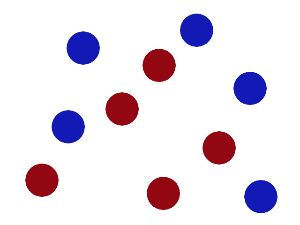
\includegraphics[width=0.5\linewidth]{partition/img/svm_7.jpg}  
%	\caption{this is a figure demo}
%	\label{fig:label}
	\end{figure}

\end{frame} 

\begin{frame}
\frametitle{一个游戏}	
现在,没有棍可以很好地分开两种球了,现在怎么办呢?我们可以一拍桌子,球飞到空中。然后,抓起一张纸,插到了两种球的中间。
           
	\begin{figure}[ht]
	\centering
	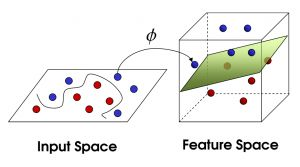
\includegraphics[width=0.5\linewidth]{partition/img/svm_8.jpg}  
%	\caption{this is a figure demo}
%	\label{fig:label}
	\end{figure}

\end{frame} 

\begin{frame}
\frametitle{一个游戏}	
现在,这些球看起来像是被一条曲线分开了。
           
	\begin{figure}[ht]
	\centering
	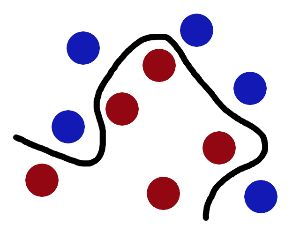
\includegraphics[width=0.5\linewidth]{partition/img/svm_9.jpg}  
%	\caption{this is a figure demo}
%	\label{fig:label}
	\end{figure}

\end{frame} 


\begin{frame}
\frametitle{怎么求解SVM?}
给定训练样本集$D = \{(x_1,y_1),(x_2,y_2),\dots,(x_m,y_m)\}$
 如果可以用一个线性超平面将其完全分开,那么这个超平面可以表示为:
\[\boldsymbol{w}^T\boldsymbol{x}+b=0\]
 其中$\boldsymbol{w}$决定了平面的方向,而b决定了平面与原点之间的距离。
           
	\begin{figure}[ht]
	\centering
	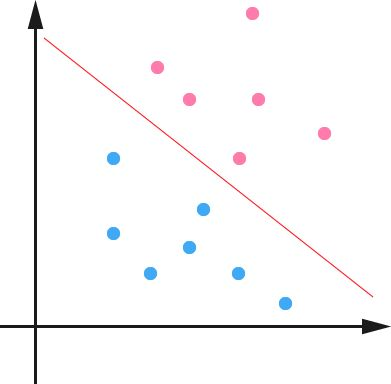
\includegraphics[width=0.5\linewidth]{partition/img/svm_10.jpg}  
%	\caption{this is a figure demo}
%	\label{fig:label}
	\end{figure}

\end{frame} 

\begin{frame}
\frametitle{间隔与支持向量}
空间中任意点$\boldsymbol{x}$实际上是一个向量,其到超平面的距离为:
\[r=\frac{\boldsymbol{w}^T\boldsymbol{x}+b}{\|\boldsymbol{w}\|}\]
	\begin{figure}[ht]
	\centering
	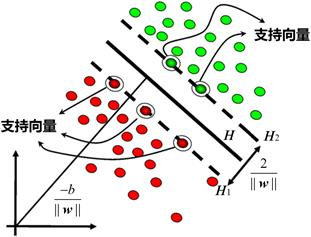
\includegraphics[width=0.5\linewidth]{partition/img/svm_11.jpg}  
%	\caption{this is a figure demo}
%	\label{fig:label}
	\end{figure}
\end{frame}

\begin{frame}
\frametitle{间隔与支持向量}
那么,如果这个超平面分类成功,我们令
\[\begin{cases}
\boldsymbol{w}^T\boldsymbol{x}+b\geq+1,\ y_i=+1\ ;\\
\boldsymbol{w}^T\boldsymbol{x}+b\leq-1,\ y_i=-1\ .
\end{cases} \]

	\begin{figure}[ht]
	\centering
	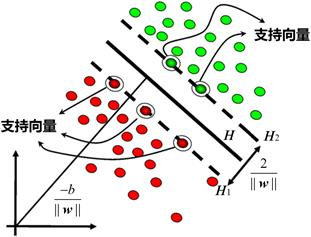
\includegraphics[width=0.5\linewidth]{partition/img/svm_11.jpg}  
%	\caption{this is a figure demo}
%	\label{fig:label}
	\end{figure}
\end{frame}

\begin{frame}
\frametitle{间隔与支持向量}

这样,那些使等号成立的点,也即距离超平面最近的点称作支持向量 (support vector),两个类到超平面距离之和也即两类之间的间隔 (margin) 是
\[
\gamma=\frac{2}{\|\boldsymbol{w}\|}
\]
训练支持向量机,实际上是希望找到具有最大间隔的划分超平面,即训练目标是在满足分类任务的情况下最大化$\gamma$,也即最大化$\|\boldsymbol{w\|}^{-1}$,也即最小化$\|\boldsymbol{w}\|^2$。
SVM的基本型就是:

\begin{gather*}
\min\limits_{\boldsymbol{w},b} \frac{1}{2}\|\boldsymbol{w}\|^2\\
s.t.\ y_i(\boldsymbol{w}^T\boldsymbol{x}_i+b)\geq1,\ i=1,2,…,m
\end{gather*}

%	\begin{figure}[ht]
%	\centering
%	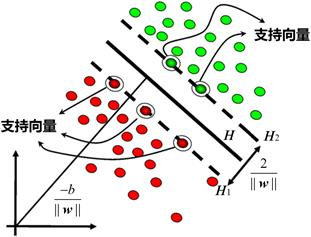
\includegraphics[width=0.3\linewidth]{partition/img/svm_11.jpg}  
%%	\caption{this is a figure demo}
%%	\label{fig:label}
%	\end{figure}
\end{frame}